% Copyright 2018-2019 Melvin Eloy Irizarry-Gelpí
\setcounter{chapter}{9}
\chapter{Interference}
%%%%%%%%%%%%%%%%%%%%%%%%%%%%%%%%%%%%%%%%%%%%%%%%%%%%%%%%%%%%%%%%%%%%%%%%%%%%%%%%
In this experiment you will learn about interference in light from a laser due to a double slit.
%%%%%%%%%%%%%%%%%%%%%%%%%%%%%%%%%%%%%%%%%%%%%%%%%%%%%%%%%%%%%%%%%%%%%%%%%%%%%%%%
\section{Preliminary}
%%%%%%%%%%%%%%%%%%%%%%%%%%%%%%%%%%%%%%%%%%%%%%%%%%%%%%%%%%%%%%%%%%%%%%%%%%%%%%%%
In the previous three experiments you studied phenomena like reflection and refraction that can be explained with the \textbf{ray} model of light. Interference and diffraction are two phenomena that are easier to explain with the \textbf{wave} model of light. Both of these have to do with light passing throw an opening or openings. But unlike the apertures you used before, the openings in this experiment and the next one are much smaller in size.

A \textbf{slit} is a very thin opening. When light goes through a single slit that is particularly narrow, a \textbf{diffraction pattern} is produced. You are going to cover diffraction in more detail in the next experiment.

A \textbf{double slit} is characterized by two distances: $a$ (the \textbf{slit width}) and $d$ (the \textbf{separation} between the two slits). When light goes through a double slit, an \textbf{interference pattern} is produced. The interference pattern consist of a series of dark and bright regions, with a very bright region in the center. The dark regions result when two waves oscillating in opposite ways meet at the same point in space (i.e. they can cancel each other, also known as \textbf{destructive} interference). The bright regions result when the two waves are oscillating in the same way (i.e. they can add to each other, also known as \textbf{constructive} interference).

Thinking of the interference pattern itself as a \textbf{wave}, the bright regions would correspond to peaks. The distance from the center of the interference pattern to the $n$-th peak is denoted by $y_{n}$. This distance $y_{n}$ is related to the distance $D$ between the screen and the double slit, the slit separation $d$, and the wavelength of the light $\lambda$ vias the relation
\begin{equation}
	\frac{y_{n} d}{\sqrt{D^{2} + y_{n}^{2}}} = n \lambda
\end{equation}
Here $n = 0$ corresponds to the central peak, $n = 1$ corresponds to the first peak, and so on. In your experiment you have the distance $D$ being much larger than the distance $y_{n}$, so you can use the following approximation:
\begin{equation}
	\sqrt{D^{2} + y_{n}^{2}} \approx D
\end{equation}
Hence it follows that the distance to a peak is given by
\begin{equation}
	y_{n} \approx \frac{n D \lambda}{d}
\end{equation}
The distance between consecutive peaks is given by
\begin{equation}
	\Delta y = y_{n+1} - y_{n} \approx \frac{D \lambda}{d}
	\label{eq.10.y}
\end{equation}
Note that this relation does not depend on the slit width $a$. The \textbf{wavelength of the red laser} used in class is 635 nm (recall that 1 nm is equivalent to $10^{-9}$ m) or $6.35 \times 10^{-4}$ mm (recall that 1 mm is equivalent to $10^{-3}$ m). Make sure that you are consistent with the units for distance.
%%%%%%%%%%%%%%%%%%%%%%%%%%%%%%%%%%%%%%%%%%%%%%%%%%%%%%%%%%%%%%%%%%%%%%%%%%%%%%%%
\section{Experiment}
%%%%%%%%%%%%%%%%%%%%%%%%%%%%%%%%%%%%%%%%%%%%%%%%%%%%%%%%%%%%%%%%%%%%%%%%%%%%%%%%
In part 1 you measure three \textbf{distances} for both the $a = 0.08$ mm single slit and $a = 0.08$ mm and $d = 0.25$ mm double slit experiment:
\begin{itemize}
	\item The distance $x_{01}$ from the middle of the central bright region to the middle of the \textbf{first dark} region.
	\item The distance $x_{02}$ from the middle of the central bright region to the middle of the \textbf{second dark} region.
	\item The distance $x_{11}$ from the middle of the first dark region in the left to the middle of the first dark region in the right.
\end{itemize}
In part 2 you measure the \textbf{intensity} along the interference pattern for three different double slits:
\begin{itemize}
	\item $a = 0.08$ mm and $d = 0.25$ mm
	\item $a = 0.04$ mm and $d = 0.25$ mm
	\item $a = 0.08$ mm and $d = 0.50$ mm
\end{itemize}
%%%%%%%%%%%%%%%%%%%%%%%%%%%%%%%%%%%%%%%%%%%%%%%%%%%%%%%%%%%%%%%%%%%%%%%%%%%%%%%%
\section{Analysis}
%%%%%%%%%%%%%%%%%%%%%%%%%%%%%%%%%%%%%%%%%%%%%%%%%%%%%%%%%%%%%%%%%%%%%%%%%%%%%%%%
Here is what to do.
%%%%%%%%%%%%%%%%%%%%%%%%%%%%%%%%%%%%%%%%%%%%%%%%%%%%%%%%%%%%%%%%%%%%%%%%%%%%%%%%
\subsection{Part 1: Distance}
%%%%%%%%%%%%%%%%%%%%%%%%%%%%%%%%%%%%%%%%%%%%%%%%%%%%%%%%%%%%%%%%%%%%%%%%%%%%%%%%
For part 1, you can compare the distance measurements for the single slit and the double slit. Although the pattern produced are very different you will find that the patterns are similar based on the distance measurements.
%%%%%%%%%%%%%%%%%%%%%%%%%%%%%%%%%%%%%%%%%%%%%%%%%%%%%%%%%%%%%%%%%%%%%%%%%%%%%%%%
\subsection{Part 2: Intensity}
%%%%%%%%%%%%%%%%%%%%%%%%%%%%%%%%%%%%%%%%%%%%%%%%%%%%%%%%%%%%%%%%%%%%%%%%%%%%%%%%
For part 2 you are only using double slits.
%%%%%%%%%%%%%%%%%%%%%%%%%%%%%%%%%%%%%%%%%%%%%%%%%%%%%%%%%%%%%%%%%%%%%%%%%%%%%%%%
\subsubsection{Visualize the data}
%%%%%%%%%%%%%%%%%%%%%%%%%%%%%%%%%%%%%%%%%%%%%%%%%%%%%%%%%%%%%%%%%%%%%%%%%%%%%%%%
Make a chart with intensity in the vertical axis and position in the horizontal axis. Instead of using the familiar ``scatter chart'', use the ``line chart'' type. Initially, your graph should look like Figure \ref{figure.10.chart1}.
%%%%%%%%%%%%%%%%%%%%%%%%%%%%%%%%%%%%%%%%%%%%%%%%%%%%%%%%%%%%%%%%%%%%%%%%%%%%%%%%
\subsubsection{Truncate the left and right tails}
%%%%%%%%%%%%%%%%%%%%%%%%%%%%%%%%%%%%%%%%%%%%%%%%%%%%%%%%%%%%%%%%%%%%%%%%%%%%%%%%
As you can see in Figure \ref{figure.10.chart1}, most of the data is just flat noise. In order to better study the central region, it is good to remove the left and right tails. For the first double slit ($a = 0.08$ mm and $d = 0.25$ mm), you can remove all the data before the pair of short peaks before the central region, and all the data after the pair of short peaks after the central region. After removing the left tail your graph will look like Figure \ref{figure.10.chart2}. After removing the right tail, the graph will look like Figure \ref{figure.10.chart3}. After these truncations, the data is ready for analysis.

For the other double slit configurations (runs 3, 4, 5, and 6), you can truncate enough to leave just the central region. Counting the central (tallest) peak, your graphs should each have 11 peaks.
%%%%%%%%%%%%%%%%%%%%%%%%%%%%%%%%%%%%%%%%%%%%%%%%%%%%%%%%%%%%%%%%%%%%%%%%%%%%%%%%
\subsubsection{Locate the position of the peaks}
%%%%%%%%%%%%%%%%%%%%%%%%%%%%%%%%%%%%%%%%%%%%%%%%%%%%%%%%%%%%%%%%%%%%%%%%%%%%%%%%
Looking at Figure \ref{figure.10.chart3}, you can clearly see a tall peak in the center. I am going to label this peak ``0C'' (``0'' for origin and ``C'' for center). On each side of 0C you can see 3 peaks of decreasing height (the third peak is very short), and a pair of peaks that appear to have the same height. I am going to label these peaks with numbers from 1 to 5 and with L if they are on the left of 0C or R if they are on the right of 0C. For Figure \ref{figure.10.chart3}, the position of these 11 peaks is in Table \ref{table.10.pos}.
%%%%%%%%%%%%%%%%%%%%%%%%%%%%%%%%%%%%%%%%%%%%%%%%%%%%%%%%%%%%%%%%%%%%%%%%%%%%%%%%
\subsubsection{Calculate the distance between adjacent peaks}
%%%%%%%%%%%%%%%%%%%%%%%%%%%%%%%%%%%%%%%%%%%%%%%%%%%%%%%%%%%%%%%%%%%%%%%%%%%%%%%%
According to the theoretical expectation, the distance between adjacent peaks is the same. To check this, you can calculate the distance between consecutive peaks. Distance is found by calculating the difference of the positions of nearby peaks. Since there are five peaks on the left, one central peak, and five peaks on the right, there is a total of ten differences. See Table \ref{table.10.disA}.
%%%%%%%%%%%%%%%%%%%%%%%%%%%%%%%%%%%%%%%%%%%%%%%%%%%%%%%%%%%%%%%%%%%%%%%%%%%%%%%%
\subsubsection{Compare to predictions}
%%%%%%%%%%%%%%%%%%%%%%%%%%%%%%%%%%%%%%%%%%%%%%%%%%%%%%%%%%%%%%%%%%%%%%%%%%%%%%%%
The data that I have been using so far was obtained with a \textbf{green} laser (you used the \textbf{red} laser). The wavelength of the green laser is 532 nm or $\lambda = 5.32 \times 10^{-4}$ mm. The distance between the slit mount and the sensor is $D = 960$ mm. For this particular run, the double slit used had $a = 0.08$ mm and $d = 0.25$ mm. With this information, the predicted separation between the peaks (\ref{eq.10.y}) takes the following value:
\begin{equation}
	\Delta y = \frac{D \lambda}{d} = \frac{(960 \text{ mm}) \times (0.000532 \text{ mm})}{(0.25 \text{ mm})} = 2.04288 \text{ mm}
\end{equation}
You can compare this expected value to the average distance between adjacent peaks found in Table \ref{table.10.disA}. The percent difference is
\begin{equation}
	\text{Percent Difference} = 100 \times \frac{2.0215 \text{ mm} - 2.04288 \text{ mm}}{2.04288 \text{ mm}} = -1.046561717 \%
\end{equation}
However, for this particular run, the distance between adjacent peaks in Table \ref{table.10.disA} varies considerably. One thing you can do is to compare the position of the peaks in Table \ref{table.10.pos} with the expected position given by multiples of the theoretical distance $\Delta y$. These results are in Table.
%%%%%%%%%%%%%%%%%%%%%%%%%%%%%%%%%%%%%%%%%%%%%%%%%%%%%%%%%%%%%%%%%%%%%%%%%%%%%%%%
\section{My Data}
%%%%%%%%%%%%%%%%%%%%%%%%%%%%%%%%%%%%%%%%%%%%%%%%%%%%%%%%%%%%%%%%%%%%%%%%%%%%%%%%
Tables \ref{table.10.part1.single} and \ref{table.10.part1.double} have the data for part 1. My intensity data contains a grand total of 15 runs. The first few runs use the green laser and I am not going to discuss them. Runs 9 to 15 use the red laser. Here is the breakdown:
\begin{itemize}
	\item Run 9 and 10: $a = 0.08$ mm and $d = 0.25$ mm
	\item Run 11 and 12: $a = 0.04$ mm and $d = 0.25$ mm
	\item Run 13 and 14: $a = 0.08$ mm and $d = 0.50$ mm
\end{itemize}
The shared spreadsheet has the analysis for runs 9 through 14. The run that I used in the text above is run 1.
%%%%%%%%%%%%%%%%%%%%%%%%%%%%%%%%%%%%%%%%%%%%%%%%%%%%%%%%%%%%%%%%%%%%%%%%%%%%%%%%
\section{Your Data}
%%%%%%%%%%%%%%%%%%%%%%%%%%%%%%%%%%%%%%%%%%%%%%%%%%%%%%%%%%%%%%%%%%%%%%%%%%%%%%%%
In part 1 you have six distance measurements. Three measurements are for the \textbf{single slit} with $a = 0.08$ mm:
\begin{itemize}
	\item The distance $x_{01}$ from the middle of the central bright region to the middle of the first dark region (both left and right; take the average).
	\item The distance $x_{02}$ from the middle of the central bright region to the middle of the second dark region (both left and right; take the average).
	\item The distance $x_{11}$ from the middle of the first dark region in the left to the middle of the first dark region in the right.
\end{itemize}
The other three measurements are for the \textbf{double slit} with $a = 0.08$ mm and $d = 0.25$ mm.

In part 2 you have six intensity measurements:
\begin{itemize}
	\item Two runs for the $a = 0.08$ and $d = 0.25$ double slit (runs 1 and 2).
	\item Two runs for the $a = 0.04$ and $d = 0.25$ double slit (runs 3 and 4).
	\item Two runs for the $a = 0.08$ and $d = 0.50$ double slit (runs 5 and 6).
\end{itemize}
%%%%%%%%%%%%%%%%%%%%%%%%%%%%%%%%%%%%%%%%%%%%%%%%%%%%%%%%%%%%%%%%%%%%%%%%%%%%%%%%
\newpage
\section{Your Lab Report}
%%%%%%%%%%%%%%%%%%%%%%%%%%%%%%%%%%%%%%%%%%%%%%%%%%%%%%%%%%%%%%%%%%%%%%%%%%%%%%%%
In your lab report you should include:
\begin{itemize}
	\item Tables like \ref{table.10.part1.single} and \ref{table.10.part1.double} with the results for part 1.
	\item An intensity versus position chart for either run 1 or run 2.
	\item An intensity versus position chart for either run 3 or run 4.
	\item An intensity versus position chart for either run 5 or run 6.
	\item A table like Table \ref{table.10.disA} for each double slit configuration. That is, either run 1 or run 2, either run 3 or run 4, and either run 5 or run 6.
	\item A table like Table \ref{table.10.results} with the average peak distance, the expected value, and the percent difference, for each of the three double slit configurations.
\end{itemize}
You should also answer the following questions:
\begin{enumerate}
	\item How do the distance measurements for the single slit and double slits in part 1 compare?
	\item Confirm that the peak separation does not depend on the slit width $a$ by comparing your results for run 1/2 and run 3/4. What happens to the average peak separation?
	\item Confirm that the peak separation depends on the slit separation $d$ by comparing your results for run 1/2 and run 5/6. What happens to the average peak separation?
	\item What do you think would happen to the interference pattern if you use a triple slit instead of a double slit?
	\item In general, are the values in your tables like Table \ref{table.10.disA} symmetric between left or right? That is, are both sides almost equally accurate? Or is one side closer to the expected values than the other?
\end{enumerate}
%%%%%%%%%%%%%%%%%%%%%%%%%%%%%%%%%%%%%%%%%%%%%%%%%%%%%%%%%%%%%%%%%%%%%%%%%%%%%%%%
\newpage
\section{Tables}
%%%%%%%%%%%%%%%%%%%%%%%%%%%%%%%%%%%%%%%%%%%%%%%%%%%%%%%%%%%%%%%%%%%%%%%%%%%%%%%%
\begin{table}[ht!]
	\centering
	\begin{tabular}{|l|r|} \hline
		Peak Label & Position (mm) \\
		\hline
		5L & 66.55 \\
		4L & 68.66 \\
		3L & 71.12 \\
		2L & 72.81 \\
		1L & 74.76 \\
		0C & 76.75 \\
		1R & 78.7 \\
		2R & 80.64 \\
		3R & 82.465 \\
		4R & 84.96 \\
		5R & 86.765 \\
		\hline
	\end{tabular}
	\caption{Positions of Peaks}
	\label{table.10.pos}
\end{table}
%%%%%%%%%%%%%%%%%%%%%%%%%%%%%%%%%%%%%%%%%%%%%%%%%%%%%%%%%%%%%%%%%%%%%%%%%%%%%%%%
\begin{table}[ht!]
	\centering
	\begin{tabular}{|l|r|} \hline
		Pair of peaks & Distance between peaks (mm) \\
		\hline
		4L -- 5L & 2.11 \\
		3L -- 4L & 2.46 \\
		2L -- 3L & 1.69 \\
		1L -- 2L & 1.95 \\
		0C -- 1L & 1.99 \\
		1R -- 0C & 1.95 \\
		2R -- 1R & 1.94 \\
		3R -- 2R & 1.825 \\
		4R -- 3R & 2.495 \\
		5R -- 4R & 1.805 \\
		\hline
		Average & 2.0215 \\
		\hline
	\end{tabular}
	\caption{Distance between adjacent peaks}
	\label{table.10.disA}
\end{table}
%%%%%%%%%%%%%%%%%%%%%%%%%%%%%%%%%%%%%%%%%%%%%%%%%%%%%%%%%%%%%%%%%%%%%%%%%%%%%%%%
\newpage
\begin{table}[ht!]
	\centering
	\begin{tabular}{|l|r|r|r|}
		\hline
		Run & Average peak separation (mm) & Expected peak separation (mm) & P.D. (\%) \\
		\hline
		1 & 2.413 & 2.413 & 0 \\
		2 & 2.404 & 2.413 & $-0.373$ \\
		3 & 2.387 & 2.413 & $-1.077$ \\
		4 & 2.384 & 2.413 & $-1.202$ \\
		5 & 1.194 & 1.2065 & $-1.036$ \\
		6 & 1.198 & 1.2065 &  $-0.705$\\
		\hline
	\end{tabular}
	\caption{Results}
	\label{table.10.results}
\end{table}
%%%%%%%%%%%%%%%%%%%%%%%%%%%%%%%%%%%%%%%%%%%%%%%%%%%%%%%%%%%%%%%%%%%%%%%%%%%%%%%%
\begin{table}[ht!]
	\centering
	\begin{tabular}{|l|r|} \hline
		Distance & Value (mm) \\
		\hline
		$x_{01}$ & 6 \\
		$x_{02}$ & 12 \\
		$x_{11}$ & 12 \\
		\hline
	\end{tabular}
	\caption{Distance measurements for the single slit for $a = 0.08$ mm.}
	\label{table.10.part1.single}
\end{table}
%%%%%%%%%%%%%%%%%%%%%%%%%%%%%%%%%%%%%%%%%%%%%%%%%%%%%%%%%%%%%%%%%%%%%%%%%%%%%%%%
\begin{table}[ht!]
	\centering
	\begin{tabular}{|l|r|} \hline
		Distance & Value (mm) \\
		\hline
		$x_{01}$ & 6 \\
		$x_{02}$ & 12 \\
		$x_{11}$ & 12 \\
		\hline
	\end{tabular}
	\caption{Distance measurements for the double slit for $a = 0.08$ mm and $d = 0.25$ mm.}
	\label{table.10.part1.double}
\end{table}
%%%%%%%%%%%%%%%%%%%%%%%%%%%%%%%%%%%%%%%%%%%%%%%%%%%%%%%%%%%%%%%%%%%%%%%%%%%%%%%%
\newpage
\section{Figures}
%%%%%%%%%%%%%%%%%%%%%%%%%%%%%%%%%%%%%%%%%%%%%%%%%%%%%%%%%%%%%%%%%%%%%%%%%%%%%%%%
\begin{figure}[ht]
	\centering
	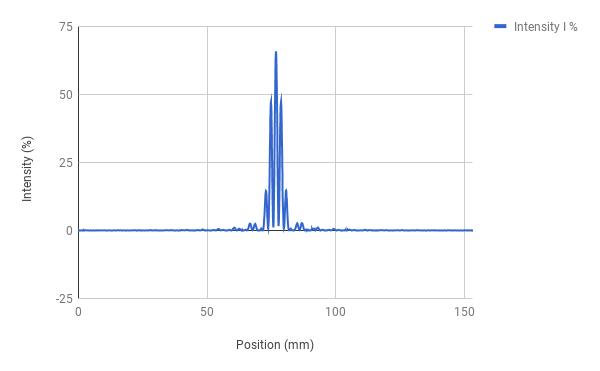
\includegraphics[scale=0.77]{image/10-interference/chart1.png}
	\caption{Intensity from interference pattern; no truncation.}
	\label{figure.10.chart1}
\end{figure}
%%%%%%%%%%%%%%%%%%%%%%%%%%%%%%%%%%%%%%%%%%%%%%%%%%%%%%%%%%%%%%%%%%%%%%%%%%%%%%%%
\begin{figure}[ht]
	\centering
	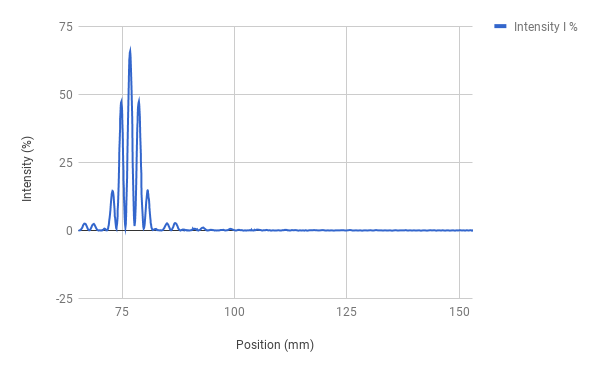
\includegraphics[scale=0.77]{image/10-interference/chart2.png}
	\caption{Intensity from interference pattern; left truncation.}
	\label{figure.10.chart2}
\end{figure}
%%%%%%%%%%%%%%%%%%%%%%%%%%%%%%%%%%%%%%%%%%%%%%%%%%%%%%%%%%%%%%%%%%%%%%%%%%%%%%%%
\begin{figure}[ht]
	\centering
	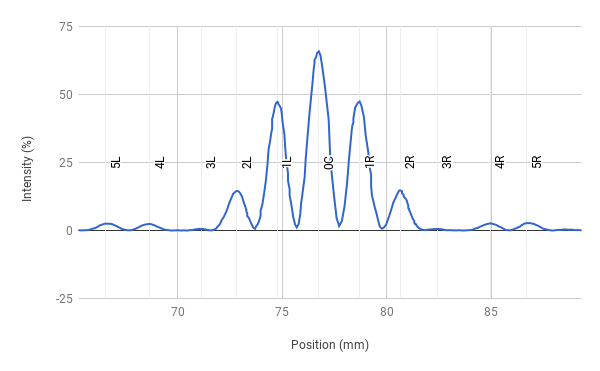
\includegraphics[scale=0.77]{image/10-interference/chart3.png}
	\caption{Intensity from interference pattern; left and right truncation.}
	\label{figure.10.chart3}
\end{figure}
%%%%%%%%%%%%%%%%%%%%%%%%%%%%%%%%%%%%%%%%%%%%%%%%%%%%%%%%%%%%%%%%%%%%%%%%%%%%%%%%